\documentclass[tikz, border=10pt]{standalone}
\usepackage{tikz}
\usepackage{amsmath}
\usepackage{amssymb}
\usepackage{xcolor}
\usetikzlibrary{arrows.meta, shapes.geometric, positioning, fit, backgrounds, calc}

\definecolor{blockBlue}{HTML}{1565c0}
\definecolor{delayOrange}{HTML}{e65100}
\definecolor{sumRed}{HTML}{c62828}
\definecolor{noiseGreen}{HTML}{2e7d32}
\definecolor{arrayGray}{HTML}{546e7a}

\tikzset{
  sigblock/.style={
    draw=blockBlue, fill=blockBlue!12, thick,
    rectangle, rounded corners=3pt,
    minimum width=1.6cm, minimum height=0.7cm,
    font=\sffamily\footnotesize, text=blockBlue
  },
  delayblock/.style={
    draw=delayOrange, fill=delayOrange!12, thick,
    rectangle,
    minimum width=1.2cm, minimum height=0.7cm,
    font=\sffamily\footnotesize, text=delayOrange
  },
  sumnode/.style={
    draw=sumRed, fill=sumRed!10, thick,
    circle, minimum size=0.7cm,
    font=\sffamily\bfseries, text=sumRed
  },
  sensor/.style={
    draw=arrayGray, fill=arrayGray!20, thick,
    circle, minimum size=0.55cm,
    font=\sffamily\footnotesize
  }
}

\begin{document}
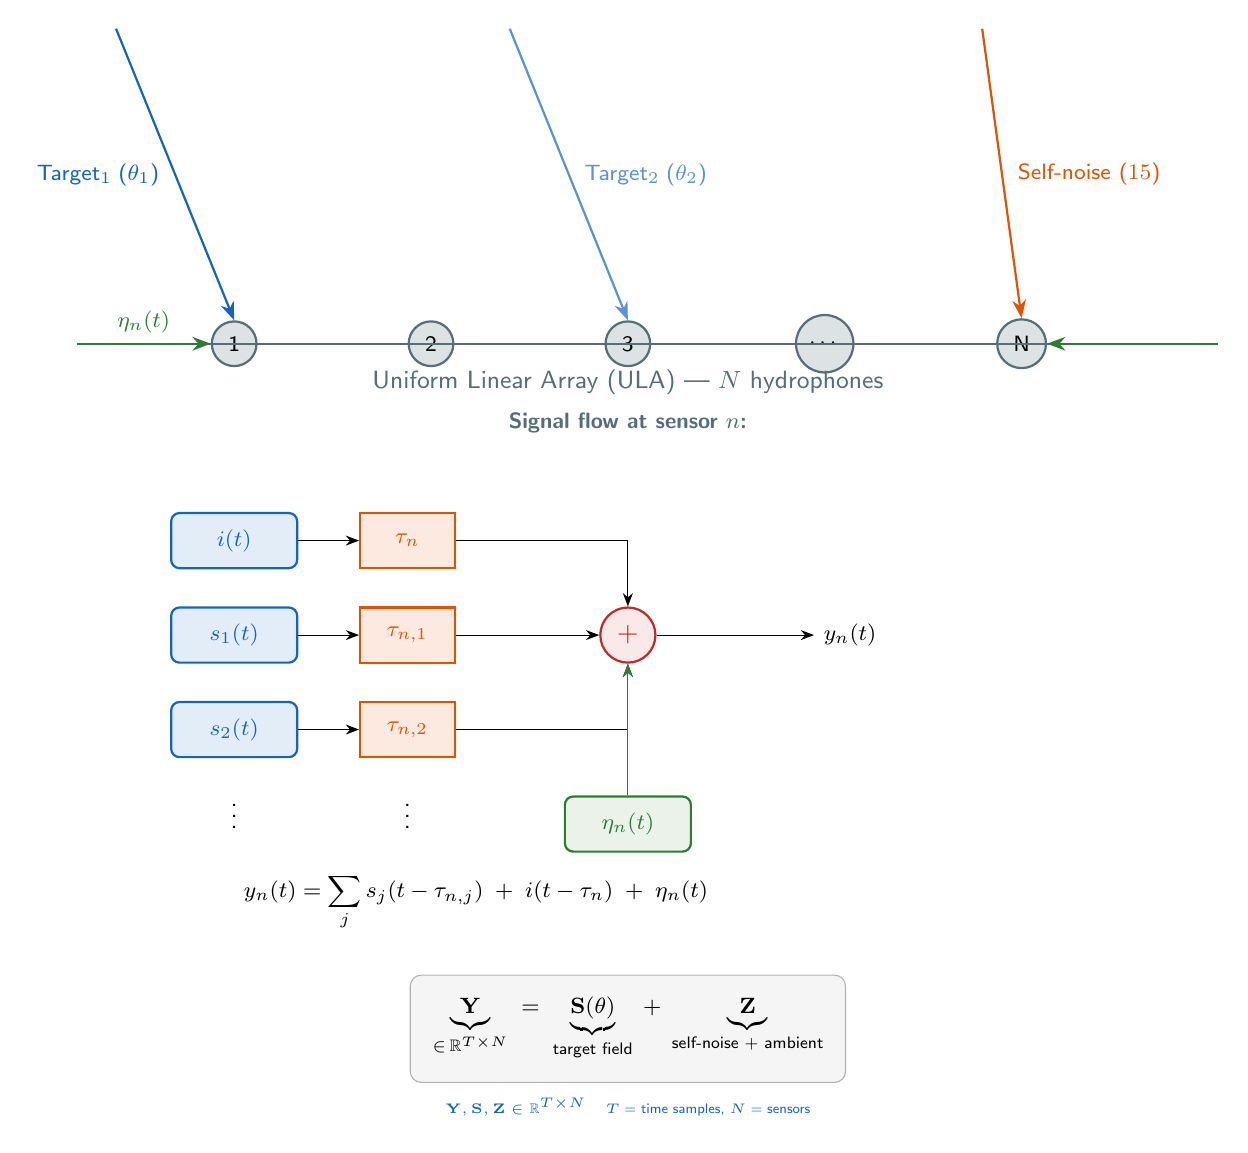
\begin{tikzpicture}[>=Stealth, font=\sffamily\small]

%% ── ULA (top section) ───────────────────────────────────────────────────
\foreach \i/\lbl in {0/1, 1/2, 2/3, 3/{$\cdots$}, 4/N}{
    \node[sensor] (s\i) at ({2.5*\i}, 5.5) {\lbl};
}
% Array baseline
\draw[arrayGray, thick]
    (-0.5, 5.5) -- ({2.5*4 + 0.5}, 5.5);
\node[arrayGray, below=6pt] at (5.0, 5.5)
    {Uniform Linear Array (ULA) — $N$ hydrophones};

%% ── Source arrows from above ────────────────────────────────────────────
% Target 1 — from upper left
\draw[blockBlue, ->, thick]
    (-1.5, 9.5) -- (s0.north)
    node[midway, left=2pt, font=\sffamily\footnotesize, blockBlue]
    {Target$_1$\;($\theta_1$)};

% Target 2 — from upper centre
\draw[blockBlue!70, ->, thick]
    (3.5, 9.5) -- (s2.north)
    node[midway, right=2pt, font=\sffamily\footnotesize, blockBlue!70]
    {Target$_2$\;($\theta_2$)};

% Self-noise — from upper right, fixed 15°
\draw[delayOrange, ->, thick]
    (9.5, 9.5) -- (s4.north)
    node[midway, right=2pt, font=\sffamily\footnotesize, delayOrange]
    {Self-noise ($15°$)};

% Ambient noise — horizontal arrows from both sides
\draw[noiseGreen, ->, thick] (-2.0, 5.5) -- (s0.west)
    node[midway, above, font=\sffamily\footnotesize, noiseGreen]
    {$\eta_n(t)$};
\draw[noiseGreen, ->, thick] (12.5, 5.5) -- (s4.east);

%% ── Signal flow for sensor n (below the array) ──────────────────────────
\node[font=\sffamily\footnotesize\bfseries, arrayGray] at (5.0, 4.5)
    {Signal flow at sensor $n$:};

% Self-noise path
\node[sigblock]  (iblock)  at (0.0, 3.0) {$i(t)$};
\node[delayblock](itau)    at (2.2, 3.0) {$\tau_n$};
\draw[->] (iblock) -- (itau);

% Target s_1 path
\node[sigblock]  (s1block) at (0.0, 1.8) {$s_1(t)$};
\node[delayblock](s1tau)   at (2.2, 1.8) {$\tau_{n,1}$};
\draw[->] (s1block) -- (s1tau);

% Target s_2 path
\node[sigblock]  (s2block) at (0.0, 0.6) {$s_2(t)$};
\node[delayblock](s2tau)   at (2.2, 0.6) {$\tau_{n,2}$};
\draw[->] (s2block) -- (s2tau);

% Ellipsis
\node at (0.0, -0.4) {$\vdots$};
\node at (2.2, -0.4) {$\vdots$};

% Summing node
\node[sumnode] (sum) at (5.0, 1.8) {$+$};

% Connect delay outputs to sum
\draw[->] (itau.east)  -| (sum.north);
\draw[->] (s1tau.east) -- (sum.west);
\draw[->] (s2tau.east) -| (sum.south);

% Ambient noise enters sum from below
\node[noiseGreen, sigblock, draw=noiseGreen, fill=noiseGreen!10,
      text=noiseGreen] (nblock) at (5.0, -0.6)
    {$\eta_n(t)$};
\draw[->, noiseGreen] (nblock.north) -- (sum.south);

% Output
\draw[->] (sum.east) -- ++(2.0, 0)
    node[right, font=\sffamily\footnotesize]
    {$y_n(t)$};

%% ── Full equation ───────────────────────────────────────────────────────
\node[font=\sffamily\footnotesize, anchor=west] at (0.0, -1.6)
    {$y_n(t) = \displaystyle\sum_j s_j\!\left(t - \tau_{n,j}\right)
      \;+\; i\!\left(t - \tau_n\right) \;+\; \eta_n(t)$};

%% ── Matrix form ─────────────────────────────────────────────────────────
\node[draw=black!30, rounded corners=4pt, fill=black!4,
      font=\sffamily\footnotesize, inner sep=8pt]
      (matbox) at (5.0, -3.2) {%
    $\underbrace{\mathbf{Y}}_{\in\,\mathbb{R}^{T\times N}}
     \;=\;
     \underbrace{\mathbf{S}(\theta)}_{\text{target field}}
     \;+\;
     \underbrace{\mathbf{Z}}_{\text{self-noise + ambient}}$
};

% Brace labels
\node[blockBlue, font=\sffamily\tiny, below=2pt] at (matbox.south)
    {$\mathbf{Y},\mathbf{S},\mathbf{Z}\in\mathbb{R}^{T\times N}$
     \quad $T$ = time samples, $N$ = sensors};

\end{tikzpicture}
\end{document}
